%% Progetto di linguaggi di programmazione - Gianluca Grilletti e Giovanni Barbarino
%% Semantica Fully Abstract per PCF


\documentclass{beamer}

\usepackage[utf8]{inputenc}
\usepackage{default}
\usepackage{amssymb}
\usepackage{stmaryrd}
\usepackage{graphicx}
\usepackage{caption}
\usepackage{xcolor}
%\usepackage{subcaption}
\usepackage{tikz}
\usetikzlibrary{arrows,automata}

\newcommand{\eqobs}{\stackrel{\text{obs}}{=}}
\newcommand{\limp}{\mathbin{{-}\mkern-3.5mu{\circ}}}


%%%% comandi tikz
\newcommand{\tnode}[4]{\node (#1_u) at (#2,#3+0.1) [minimum size=2pt, opacity=0]{#4};
		       \node (#1_d) at (#2,#3-0.1) [minimum size=2pt, opacity=0] {#4};
		       \node (#1) at (#2,#3) [minimum size=2pt] {#4};}



% immagini
\graphicspath{{immagini/}}




\usetheme{Darmstadt}
\setbeamercovered{dynamic}

\title{Un modello fully abstract del PCF}
% \subtitle{Vuoi fare un gioco con me?}
\author{Grilletti Gianluca \and Barbarino Giovanni}
\institute[Unipi]{Università di Pisa}


\begin{document}

\small


%titolo
\begin{frame}
	%\frametitle{Il linguaggio PCF}
	\maketitle
	
\end{frame}

\section{La categoria dei giochi}


\subsection{giochi e strategie}

% i giochi
\begin{frame}
	\frametitle{I giochi}
	
	Il modello che andremo a considerare si basa sulla \emph{teoria dei giochi}.
	
	
	Un \textbf{gioco} è una 4-upla $A=( M_A , \lambda_A , P_A , \approx_A )$ dove:
	\begin{itemize}
	\item<2-> $M_A$ è l'insieme delle mosse
	\item<3-> $\lambda_A$ è una funzione da $M_A$ all'insieme $\{ O,P\} \times \{Q,A\}$; in particolare:
		\begin{itemize}
		\item $O$ indica il giocatore "opponent" e $P$ il giocatore "player"
		\item $Q$ indica una domanda e $A$ una risposta
		\end{itemize}
	\item<4-> Una \textit{partita} è una stringa finita di mosse tale che:
		\begin{enumerate}
		\item La prima mossa è di $O$
		\item $P$ e $O$ si alternano
		\item In ogni sottostringa iniziale, il numero di risposte deve essere al più uguale al numero di domande (\emph{bracketing condition})
		\end{enumerate}
	\item<5-> $P_A$ è un sottoinsieme prefix-closed di partite; chiameremo $P_A$ l'insieme delle \textit{partite valide}
	\item<6->  $\approx_A$ è una relazione di equivalenza sulle partite valide
	\end{itemize}
	
	
\end{frame}

% tavolo e carte
\begin{frame}

\frametitle{Tavolo di Gioco}
	
	Possiamo rappresentare partite accettabili tramite il \emph{Tavolo di Gioco}
	
	\begin{columns}
	\begin{column}{0.45\textwidth}
	\only<2->{Gioco $A=( M_A , \lambda_A , P_A , \approx_A )$
		\begin{itemize}
		         	\item $M_{A}=\{*_1,*_2,n_1,n_2\}$
		           	\item $\lambda_{A}= \{ (*_1,OQ) ;$ $ (*_2,PQ) ; (n_1,PA) ; (n_2,OA) \}$
					\item $P_{A}= \{ 
					\only<3>{\textcolor{red}}{\epsilon} ,$
					$ \only<4>{\textcolor{red}}{*_1} ,
					\; *_1n_1, $ 
					$ \only<5>{\textcolor{red}}{*_1*_2},
					\; \only<6>{\textcolor{red}}{*_1*_2n_2}, 
					\; \only<7>{\textcolor{red}}{*_1*_2n_2n_1} \}$
					\item $\approx_{A} = id_{A}$        
		\end{itemize}}
	\end{column}
	\begin{column}{0.4\textwidth}
		\begin{tikzpicture}
			 \node (inv) at (0,0) [minimum size=2pt] {};
			 \node (inv2) at (4,-5) [minimum size=2pt, scale=1.5] {};
			 
	\only<3->{	 \draw [fill=blue, opacity=.5] (3.5,-4) rectangle (.5,-1);
			 \node (A) at (2,-2.5) [minimum size=2pt, scale=4] {A};
			 \node (P) at (1,-3.5) [minimum size=2pt, scale=2.5] {P};
			 \node (O) at (1,-1.5) [minimum size=2pt, scale=2.5] {O};}
			 
			 
			 
			 \only<4-> {\node (st_1) at (2.5,-.5) [minimum size=2pt, scale=1.5] {$*_1$};}
			 \only<5-> {\node (st_2) at (2.5,-4.5) [minimum size=2pt, scale=1.5] {$*_2$};}
			 \only<6->{\node (ri_1) at (1.5,-.5) [minimum size=2pt, scale=1.5] {$n_2$};}
			 \only<7->{\node (ri_2) at (1.5,-4.5) [minimum size=2pt, scale=1.5] {$n_1$};}
			 
			  \only<5->{\draw[->] [out=280,in=80] (st_1) to (st_2);}
			  \only<6->{\draw[->] [out=110,in=300] (st_2) to (ri_1);}
			  \only<7->{\draw[->] [out=280,in=80] (ri_1) to (ri_2);}
			  
			\end{tikzpicture}
		
	\end{column}
	\end{columns}

	%\only<8> {\centering
	%Solo $P$ può rispondere alle domande di $O$, e viceversa}
	
\end{frame}



% strategie
\begin{frame}

	\frametitle{Strategie}
	
	Una \textbf{strategia} $\sigma$ è un insieme di partite di lunghezza pari (l'ultima mossa è di $P$) tali che:
	\begin{itemize}
		\item<2-> $\sigma$ sia prefix-closed sulle partite di lunghezza pari
		\item<3-> $\sigma$ sia \textit{history free}, cioè
		\begin{itemize}
			\item $sab , tac \in \sigma \Rightarrow b=c$
			\item $sab, t\in \sigma, ta\in P_A \Rightarrow tab\in \sigma$
		\end{itemize}
	\end{itemize}
	
	
	\onslide<4> 
	La condizione di history free, rende le strategie esprimibili tramite una \textit{funzione parziale} a loro associata:
	\begin{gather*}
		    f: M^O \rightharpoonup M^P\\
	            sab\in \sigma \Rightarrow f_\sigma(a)=b\\
	            X=\{ab\;|\;f(a)=b\} \rightarrow \sigma_f=<X> 
	\end{gather*}
	
	
\end{frame}

% esempi di strategie
\begin{frame}

\frametitle{Strategie}

	\begin{columns}
	\begin{column}{0.45\textwidth}
	Gioco $A=( M_A , \lambda_A , P_A , \approx_A )$
		\begin{itemize}
		         	\item $M_{A}=\{*_1,*_2,n_1,n_2\}$
		           	\item $\lambda_{A}= \{ (*_1,OQ) ;$ $ (*_2,PQ) ; (n_1,PA) ; (n_2,OA) \}$
					\item $P_{A}= \{ 
					\epsilon ,$
					$ *_1 ,
					\; *_1n_1, $ 
					$ *_1*_2,
					\; *_1*_2n_2, 
					\; *_1*_2n_2n_1 \}$
					\item $\approx_{A} = id_{A}$        
		\end{itemize}
	\end{column}
	\begin{column}{0.4\textwidth}
		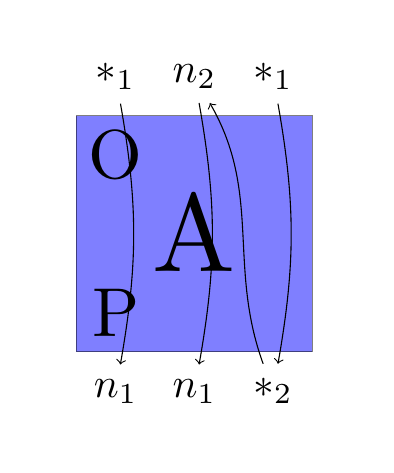
\begin{tikzpicture}
			 \node (inv) at (0,0) [minimum size=2pt] {};
			 \node (inv2) at (4,-5) [minimum size=2pt, scale=1.5] {};
			 
			 \draw [fill=blue, opacity=.5] (3.5,-4) rectangle (.5,-1);
			 \node (A) at (2,-2.5) [minimum size=2pt, scale=4] {A};
			 \node (P) at (1,-3.5) [minimum size=2pt, scale=2.5] {P};
			 \node (O) at (1,-1.5) [minimum size=2pt, scale=2.5] {O};
			 
			 \only<2>{
			 \node (st_12) at (1,-.5) [minimum size=2pt, scale=1.5] {$*_1$};
			 \node (ri_12) at (1,-4.5) [minimum size=2pt, scale=1.5] {$n_1$};
		
			 
			 \node (st_1) at (3,-.5) [minimum size=2pt, scale=1.5] {$*_1$};
			 \node (st_2) at (3,-4.5) [minimum size=2pt, scale=1.5] {$*_2$};
			 \node (ri_1) at (2,-.5) [minimum size=2pt, scale=1.5] {$n_2$};
			 \node (ri_2) at (2,-4.5) [minimum size=2pt, scale=1.5] {$n_1$};
			 
			  \draw[->] [out=280,in=80] (st_1) to (st_2);
			  \draw[->] [out=110,in=300] (st_2) to (ri_1);
			  \draw[->] [out=280,in=80] (ri_1) to (ri_2);
			  \draw[->] [out=280,in=80] (st_12) to (ri_12);
			}
			\end{tikzpicture}
		
	\end{column}
	\end{columns}
	\centering
	\onslide<2>
	Esempi di strategie:
	\begin{gather*}
	\sigma=\{\epsilon, *_1n_1\}\leftrightarrow f_\sigma(*_1)=n_1  \\
	\tau=\{\epsilon, \; *_1*_2, \; *_1*_2n_2n_1\}\leftrightarrow f_\tau(*_1)=*_2,\; f_\tau(n_2)=n_1
	\end{gather*}
	
\end{frame}

\begin{frame}
 
 Estendiamo la relazione $\approx$ alle strategie, ponendo:
 \pause
	\begin{itemize}
	\item $\underline{ \sigma \preccurlyeq_s \tau }$ se per ogni $sab \in \sigma$ e $s' \in \tau$ t.c. $sa\approx s'a'$, esiste $b'$ tale che $s'a'b' \in \tau$ e $sab\approx s'a'b'$
	\item $\underline{ \sigma \approx_s \tau \ } \; \text{sse} \; \sigma \preccurlyeq_s \tau \wedge \tau \preccurlyeq_s \sigma$
	\end{itemize}  
	\pause
In particolare, la definizione porta alcune conseguenze: 

	\begin{itemize}
		\item $\preccurlyeq_s$ è un preordine sulle strategie; di conseguenza $\approx_s$ è una relazione di equivalenza parziale
		\item Nel caso l'equivalenza $\approx$ del gioco sia l'identità, l'ordine tra strategie si può vedere come inclusione di insiemi o tra le funzioni parziali. Intuitivamente, $\sigma \preccurlyeq_s \tau$ se $\tau$ può fare più mosse di $\sigma$
	\end{itemize}
	
\end{frame}

\begin{frame}
	\begin{columns}
	\begin{column}{0.45\textwidth}
	Gioco $A=( M_A , \lambda_A , P_A , \approx_A )$
		\begin{itemize}
		         	\item $M_{A}=\{*_1,*_2,n_1,n_2\}$
		           	\item $\lambda_{A}= \{ (*_1,OQ) ;$ $ (*_2,PQ) ; (n_1,PA) ; (n_2,OA) \}$
					\item $P_{A}= \{ 
					\epsilon ,$
					$ *_1 ,
					\; *_1n_1, $ 
					$ *_1*_2,
					\; *_1*_2n_2, 
					\; *_1*_2n_2n_1 \}$
					\item $\approx_{A} = id_{A}$        
		\end{itemize}
	\end{column}
	\begin{column}{0.4\textwidth}
		\begin{tikzpicture}
			 \node (inv) at (0,0) [minimum size=2pt] {};
			 \node (inv2) at (4,-5) [minimum size=2pt, scale=1.5] {};
			 
			 \draw [fill=blue, opacity=.5] (3.5,-4) rectangle (.5,-1);
			 \node (A) at (2,-2.5) [minimum size=2pt, scale=4] {A};
			 \node (P) at (1,-3.5) [minimum size=2pt, scale=2.5] {P};
			 \node (O) at (1,-1.5) [minimum size=2pt, scale=2.5] {O};
			 
			 \node (st_12) at (1,-.5) [minimum size=2pt, scale=1.5] {$*_1$};
			 \only<1-2>{\node (ri_12) at (1,-4.5) [minimum size=2pt, scale=1.5] {$n_1$};}
	 		 \only<3-4>{\node (st_22) at (1,-4.5) [minimum size=2pt, scale=1.5] {$*_2$};}
			 \node (st_1) at (3,-.5) [minimum size=2pt, scale=1.5] {$*_1$};
			 \node (st_2) at (3,-4.5) [minimum size=2pt, scale=1.5] {$*_2$};
			 \node (ri_1) at (2,-.5) [minimum size=2pt, scale=1.5] {$n_2$};
			 \node (ri_2) at (2,-4.5) [minimum size=2pt, scale=1.5] {$n_1$};
			 
			  \draw[->] [out=280,in=80] (st_1) to (st_2);
			  \draw[->] [out=110,in=300] (st_2) to (ri_1);
			  \draw[->] [out=280,in=80] (ri_1) to (ri_2);
			  \only<1-2>{\draw[->] [out=280,in=80] (st_12) to (ri_12);}
			  \only<3-4>{\draw[->] [out=280,in=80] (st_12) to (st_22);}
			\end{tikzpicture}
		
	\end{column}
	\end{columns}
	\centering
	\begin{gather*}
	\only<1-2>{\sigma=\{\epsilon, *_1n_1\}\leftrightarrow f_\sigma(*_1)=n_1  \\}
	\only<3-4>{\sigma=\{\only<4>{\textcolor{red}{\epsilon, \; *_1*_2}}\only<3>{\epsilon, \; *_1*_2}\}\leftrightarrow \only<4>{\textcolor{red}{f_\sigma(*_1)=*_2}}\only<3>{f_\sigma(*_1)=*_2}  \\}
	\tau=\{\only<4>{\textcolor{red}{\epsilon, \; *_1*_2}}\only<1-3>{\epsilon, \; *_1*_2}, \; *_1*_2n_2n_1\}\leftrightarrow 
	\only<4>{\textcolor{red}{f_\tau(*_1)=*_2}}\only<1-3>{f_\tau(*_1)=*_2},\; 
	f_\tau(n_2)=n_1
	\\
	\only<2>{\sigma \not\preccurlyeq_s \tau, \; \sigma \not\preccurlyeq_s \tau}
	\only<4>{\sigma \preccurlyeq_s \tau}
	\end{gather*}
\end{frame}

\subsection{operazioni tra giochi}

% prodotto tensore
\begin{frame}
	
	\frametitle{Il gioco $A \otimes B$}
	
	\begin{itemize}
		\item $M_{A\otimes B}=M_A \coprod M_B$
		\item $\lambda_{A\otimes B}=\lambda_A \coprod \lambda_B$
		\item $P_{A\otimes B}$ sono tutte le partite $s$ tali che $s|_{M_A} \in P_A \wedge s|_{M_B} \in P_B$
		%\begin{itemize}
			
		%	\item Per ogni domanda in $A$, la risposta deve essere in $A$; lo stesso con $B$
		%\end{itemize}
		\item $s\approx_{A\otimes B} t \Leftrightarrow s|_A \approx_A t|_A \wedge s|_B \approx_B t|_B \wedge fst(s)=fst(t)$ 
	\end{itemize}
	
	\begin{block}{Proprietà}
		\begin{itemize}
			\item Il prodotto tensore è associativo
			\item Esiste un elemento neutro $I$, ossia il gioco vuoto
			\item Solamente il giocatore $O$ può cambiare componente di gioco
		\end{itemize}
		
	\end{block}
	
	
\end{frame}


\begin{frame}[t]
	
% 	\begin{tabular}{c c}
% 		
% 		
% 		%%%%%%% TAVOLO 1
% 		\only<2>{$\textcolor{red}{*^O_A}$}\only<3->{$*^O_A$}
% 		&
% 		%%%%%%% TAVOLO 2
% 		\only<4>{$\textcolor{red}{*^O_B}$}\only<5->{$*^O_B$}
% 		\\
% 		
% 		\begin{minipage}{0.48\textwidth}
% 			\begin{figure}[t]
% 				\Large
% 				\centering
% 				\def\svgwidth{0.6\textwidth}
% 				\input{immagini/tavolo_a.pdf_tex}
% 			\end{figure}
% 		\end{minipage} &  \begin{minipage}{0.48\textwidth}
% 			\begin{figure}[t]
% 				\Large
% 				\centering
% 				\def\svgwidth{0.6\textwidth}
% 				\input{immagini/tavolo_b.pdf_tex}
% 			\end{figure}
% 		\end{minipage} \\
% 		
% 		%%%%%%% TAVOLO 1
% 		\only<3>{$\textcolor{red}{n^P_A}$}\only<4->{$n^P_A$}
% 		&
% 		%%%%%%% TAVOLO 2
% 		\only<5->{$\textcolor{red}{m^P_B}$}
% 		
% 		
% 	\end{tabular}
% 	
% 	
% 	{
% 	\centering
% 	\huge
% 	
% 	
% 	\onslide<2->{\only<-2>{$\textcolor{red}{*^O_A}$}\only<3->{$*^O_A$}}
% 	\onslide<3->{\only<-3>{$\textcolor{red}{n^P_A}$}\only<4->{$n^P_A$}}
% 	\onslide<4->{\only<-4>{$\textcolor{red}{*^O_B}$}\only<5->{$*^O_B$}}
% 	\onslide<5->{\only<-5>{$\textcolor{red}{m^P_B}$}}
% 
% 	
% 	
% 	}
	
\end{frame}


% gioco implicazione lineare
\begin{frame}
	
	\frametitle{Il gioco $A \limp B$}
	
	\begin{itemize}
		\item $M_{A\limp B}=M_A \coprod M_B$
		\item $\lambda^{QA}_{A\limp B}=\lambda^{QA}_A \coprod \lambda^{QA}_B$
		
		$\lambda^{OP}_{A\limp B}=\overline{\lambda^{OP}_A} \coprod \lambda^{OP}_B$
		\item $P_{A\otimes B}$ sono tutte le partite $s$ tali che:
		\begin{itemize}
			\item $s|_{M_A} \in P_A \wedge s|_{M_B} \in P_B$
			\item Per ogni domanda in $A$, la risposta deve essere in $A$; lo stesso con $B$
		\end{itemize}
		\item $s\approx_{A\otimes B} t \Leftrightarrow s|_A \approx_A t|_A \wedge s|_B \approx_B t|_B \wedge fst(s)=fst(t)$ 
	\end{itemize}
	
	\begin{block}{Proprietà}
		
		\begin{itemize}
			\item Solamente il giocatore $P$ può cambiare componente di gioco
		\end{itemize}
	
	\end{block}
	
\end{frame}


\begin{frame}[t]
	
% 	\begin{tabular}{c c}
% 		
% 		%%%%%%% TAVOLO 1
% 		\only<3>{$\textcolor{red}{*^P_A}$}\only<4->{$*^P_A$}
% 		&
% 		%%%%%%% TAVOLO 2
% 		\only<2>{$\textcolor{red}{*^O_B}$}\only<3->{$*^O_B$}
% 		\\
% 		
% 		\begin{minipage}{0.48\textwidth}
% 			\begin{figure}[t]
% 				\Large
% 				\centering
% 				\def\svgwidth{0.6\textwidth}
% 				\input{immagini/tavolo_a_storto.pdf_tex}
% 			\end{figure}
% 		\end{minipage} &  \begin{minipage}{0.48\textwidth}
% 			\begin{figure}[t]
% 				\Large
% 				\centering
% 				\def\svgwidth{0.6\textwidth}
% 				\input{immagini/tavolo_b.pdf_tex}
% 			\end{figure}
% 		\end{minipage} \\
% 		
% 		%%%%%%% TAVOLO 1
% 		\only<4>{$\textcolor{red}{n^O_A}$}\only<5->{$n^O_A$}
% 		&
% 		%%%%%%% TAVOLO 2
% 		\only<5->{$\textcolor{red}{m^P_B}$}
% 		
% 		
% 	\end{tabular}
% 	
% 	
% 	{
% 	\centering
% 	\huge
% 	
% 	
% 	\onslide<2->{\only<-2>{$\textcolor{red}{*^O_B}$}\only<3->{$*^O_B$}}
% 	\onslide<3->{\only<-3>{$\textcolor{red}{*^P_A}$}\only<4->{$*^P_A$}}
% 	\onslide<4->{\only<-4>{$\textcolor{red}{n^O_A}$}\only<5->{$n^O_A$}}
% 	\onslide<5->{\only<-5>{$\textcolor{red}{m^P_B}$}}
% 	
% 	
% 	
% 	}
	
	
\end{frame}

% gioco unione
\begin{frame}
	
	\frametitle{Il gioco $A \& B$}
	
	\begin{itemize}
		\item $M_{A\& B}=M_A \coprod M_B$
		\item $\lambda_{A\& B}=\lambda_A \coprod \lambda_B$
		\item $P_{A\& B}=P_A \coprod P_B$
		\item $\approx_{A\& B} \; = \; \approx_A \coprod \approx_B$ 
	\end{itemize}
	
	\begin{block}{Proprietà}
		\begin{itemize}
			\item Una partita di $A\& B$ è giocata su una sola delle due componenti
			\item Ogni strategia di $A\& B$ è unione di una strategia di $A$ e di una strategia di $B$
		\end{itemize}
		
	\end{block}
	
\end{frame}


\begin{frame}[t]
	
% 	\begin{tabular}{c c}
% 		
% 		%%%%%%% TAVOLO 1
% 		\only<2>{$\textcolor{red}{*^O_A}$}\only<3->{$*^O_A$}
% 		&
% 		%%%%%%% TAVOLO 2
% 		
% 		
% 		\\
% 		
% 		\begin{minipage}{0.48\textwidth}
% 			\begin{figure}[t]
% 				\Large
% 				\centering
% 				\def\svgwidth{0.6\textwidth}
% 				\input{immagini/tavolo_a.pdf_tex}
% 			\end{figure}
% 		\end{minipage} &  \begin{minipage}{0.48\textwidth}
% 			\begin{figure}[t]
% 				\Large
% 				\centering
% 				\def\svgwidth{0.6\textwidth}
% 				\input{immagini/tavolo_b.pdf_tex}
% 			\end{figure}
% 		\end{minipage} \\
% 		
% 		%%%%%%% TAVOLO 1
% 		\only<3>{$\textcolor{red}{n^P_A}$}
% 		&
% 		%%%%%%% TAVOLO 2
% 		
% 		
% 	\end{tabular}
% 	
% 	
% 	{
% 	\centering
% 	\huge
% 	
% 
% 	\onslide<2->{\only<-2>{$\textcolor{red}{*^O_A}$}\only<3->{$*^O_A$}}
% 	\onslide<3->{\only<-3>{$\textcolor{red}{n^P_A}$}}
% 
% 	
% 	
% 	}
% 	
	
\end{frame}

% gioco prodotto tensore infinito
\begin{frame}
	
	\frametitle{Il gioco $!A$}
	
	\begin{itemize}
		\item $M_{!A}=\omega \times M_A$
		\item $\lambda_{!A}(i,a)=\lambda_A(a)$
		\item $s$ è una partita di $P_{!A}$ se e solo se:
		\begin{itemize}
			\item $\forall i\in \omega , s|_i \in P_A$
			\item Se una domanda è nella componente $i$, la sua risposta deve essere nella componente $i$ (\emph{indexed bracketing condition})
		\end{itemize}

		\item $s\approx_{!A} t$ sse esiste $\pi:\omega \rightarrow \omega$ permutazione tale che $s|_i \approx_A t|_{\pi(i)} \wedge (\pi \circ fst)(s)=fst(t)$
	\end{itemize}
	
	\begin{block}{Proprietà}
		\begin{itemize}
			\item Solamente il giocatore $O$ può cambiare componente di gioco
		\end{itemize}
	\end{block}
	
	Nota: concettualmente il gioco $!A$ si comporta come se avessimo infinite copie di $A$ tensorizzate $A\otimes A\otimes A\otimes A\otimes \dots$
	
\end{frame}


\begin{frame}[t]
	
% 	\begin{tabular}{c c c c}
% 		
% 		%%%%%%% TAVOLO 1
% 		
% 		&
% 		%%%%%%% TAVOLO 2
% 		\only<8>{$\textcolor{red}{*^O_3}$}\only<9->{$*^O_3$}
% 		&
% 		%%%%%%% TAVOLO 3
% 		\only<4>{$\textcolor{red}{*^O_2}$}\only<5->{$*^O_2$}
% 		&
% 		%%%%%%% TAVOLO 4
% 		\only<2>{$\textcolor{red}{*^O_1}$}\only<3->{$*^O_1$}\onslide<6->{\only<-6>{$\textcolor{red}{*^O_1}$}\only<7->{$*^O_1$}}
% 		
% 		\\
% 		
% 		\begin{minipage}{0.22\textwidth}
% 			\begin{figure}[t]
% 				\large
% 				\centering
% 				\def\svgwidth{0.8\textwidth}
% 				\input{immagini/tavolo_a_4.pdf_tex}
% 			\end{figure}
% 		\end{minipage} &  \begin{minipage}{0.22\textwidth}
% 			\begin{figure}[t]
% 				\large
% 				\centering
% 				\def\svgwidth{0.8\textwidth}
% 				\input{immagini/tavolo_a_3.pdf_tex}
% 			\end{figure}
% 		\end{minipage} & \begin{minipage}{0.22\textwidth}
% 			\begin{figure}[t]
% 				\large
% 				\centering
% 				\def\svgwidth{0.8\textwidth}
% 				\input{immagini/tavolo_a_2.pdf_tex}
% 			\end{figure}
% 		\end{minipage} & \begin{minipage}{0.22\textwidth}
% 			\begin{figure}[t]
% 				\large
% 				\centering
% 				\def\svgwidth{0.8\textwidth}
% 				\input{immagini/tavolo_a_1.pdf_tex}
% 			\end{figure}
% 		\end{minipage} \\
% 		
% 		%%%%%%% TAVOLO 1
% 		
% 		&
% 		%%%%%%% TAVOLO 2
% 		\only<9>{$\textcolor{red}{n^P_3}$}
% 		&
% 		%%%%%%% TAVOLO 3
% 		\only<5>{$\textcolor{red}{n^P_2}$}\only<6->{$n^P_2$}
% 		&
% 		%%%%%%% TAVOLO 4
% 		\only<3>{$\textcolor{red}{n^P_1}$}\only<4->{$n^P_1$}\onslide<7->{\only<-7>{$\textcolor{red}{n^P_1}$}\only<8->{$n^P_1$}}
% 		
% 	\end{tabular}
% 	
% 	
% 	{
% 	\centering
% 	\huge
% 	
% 	\onslide<2->{\only<-2>{$\textcolor{red}{*^O_1}$}\only<3->{$*^O_1$}}
% 	\onslide<3->{\only<-3>{$\textcolor{red}{n^P_1}$}\only<4->{$n^P_1$}}
% 	\onslide<4->{\only<-4>{$\textcolor{red}{*^O_2}$}\only<5->{$*^O_2$}}
% 	\onslide<5->{\only<-5>{$\textcolor{red}{n^P_2}$}\only<6->{$n^P_2$}}
% 	\onslide<6->{\only<-6>{$\textcolor{red}{*^O_1}$}\only<7->{$*^O_1$}}
% 	\onslide<7->{\only<-7>{$\textcolor{red}{n^P_1}$}\only<8->{$n^P_1$}}
% 	\onslide<8->{\only<-8>{$\textcolor{red}{*^O_3}$}\only<9->{$*^O_3$}}
% 	\onslide<9->{\only<-9>{$\textcolor{red}{n^P_3}$}}
% 	
% 	}
	
	
\end{frame}

\subsection{strategie importanti}

% esempi di strategie
\begin{frame}

	\frametitle{Alcune strategie}
	
	DOBBIAMO DECIDERE COME SPIEGARE LE STRATEGIE; QUESTE ANDREBBERO DETTE:
	\begin{itemize}
		\item $\sigma ; \tau$ [NO]
		\item $id_{A\limp A}$ (la copy-cat) [SI]
		\item $App:(A \Rightarrow B)\& A \Rightarrow B$ [SI]
	\end{itemize}

\end{frame}


\begin{frame}[t]
	
% 	\frametitle{La strategia copycat}
% 	
% 	\begin{tabular}{c c}
% 		
% 		%%%%%%% TAVOLO 1
% 		
% 		&
% 		%%%%%%% TAVOLO 2
% 		
% 		\\
% 		
% 		\begin{minipage}{0.48\textwidth}
% 			\begin{figure}[t]
% 				\Large
% 				\centering
% 				\def\svgwidth{0.6\textwidth}
% 				\input{immagini/tavolo_a_storto.pdf_tex}
% 			\end{figure}
% 		\end{minipage} &  \begin{minipage}{0.48\textwidth}
% 			\begin{figure}[t]
% 				\Large
% 				\centering
% 				\def\svgwidth{0.6\textwidth}
% 				\input{immagini/tavolo_a.pdf_tex}
% 			\end{figure}
% 		\end{minipage} \\
% 		
% 		%%%%%%% TAVOLO 1
% 		
% 		&
% 		%%%%%%% TAVOLO 2
% 		
% 		
% 	\end{tabular}
	

	
\end{frame}

\subsection{esistenza del modello}

% categoria dei giochi
\begin{frame}
 	
 	\frametitle{La categoria dei giochi $\mathcal{G}$}
 	
 	Definiamo $\mathcal{G}$ la categoria tale che:
 	\begin{itemize}
 		\item $\mathcal{G}_0$ sono i giochi
 		\item dati due giochi $A$ e $B$, i morfismi $A\rightarrow B$ sono $\{ \sigma \text{ strategia di } A\limp B | \sigma \approx \sigma \} / \approx$
 		\item Date $[\sigma] : A\rightarrow B$ e $[\tau] : B \rightarrow C$, $[\tau] \circ [\sigma] = [\sigma ; \tau]$
 	\end{itemize}
 	
 	In particolare $\mathcal{G}$ è dotata di:
 	\begin{itemize}
 		\item un oggetto finale ($1$)
 		\item è una categoria monoidale (è definito $\otimes$ bifuntore associativo e con elemento neutro)
 		\item è una categoria autonoma (per ogni gioco $A$ esiste il suo gioco duale $1 \limp A$)
 		\item NON è una categoria cartesiana chiusa (mancano i prodotti)
 	\end{itemize}
 	
 \end{frame}

% categoria di co-Kleisli
\begin{frame}

Definiamo $K_!(\mathcal{G})$ la categoria di \emph{co-Kleisli} di $\mathcal{G}$ rispetto a $!$; in particolare:
	
	\begin{itemize}
		\item $K_!(\mathcal{G})_0 = \mathcal{G}_0$
		\item Dati due giochi $A,B$, $Mor_{K_!(\mathcal{G})}(A,B) = Mor_{\mathcal{G}}(!A,B)$
		\item Date due strategie $\sigma$ e $\tau$, $\tau \circ \sigma = \sigma \fatsemi \tau = \sigma ^\dag ; \tau$
		\item Dato un gioco $A$, il morfismo identico è $der_A$
	\end{itemize}

	In particolare $K_!(\mathcal{G})$ è una \emph{categoria cartesiana chiusa}, cioè:
	\begin{itemize}
		\item Dati due oggetti esiste il \emph{prodotto} ($A\& B$)
		\item Esiste un oggetto \emph{finale} ($1$)
		\item Dati due oggetti, esiste l'oggetto esponente 
		
		(l'operatore ``$\Rightarrow$'' è tale che $Mor(A\& B,C) \cong Mor(A,B\Rightarrow C)$)
	\end{itemize}

\end{frame}

% ppo e ccc razionale
\begin{frame}
	
	\frametitle{order enrichement}
	
	Definiamo un \emph{pointed poset (ppo)} come un poset con un minimo (generalmente indicato con $\perp$)
	
	Definiamo una categoria cartesiana chiusa $C$ \emph{pointed poset enriched} se:
	\begin{itemize}
		\item Dati due oggetti $A,B$, $(Mor(A,B),\sqsubseteq _{A,B},\perp _{A,B})$ è un pointed poset
		\item Composizione, prodotto e currying sono monotoni
		\item Per ogni $f: A\rightarrow B$, per ogni gioco $C$, $\perp_{B,C} \circ f = \perp _{A,B}$
	\end{itemize}
	
	Definiamo una categoria cartesiana chiusa $C$ \emph{razionale} se:
	\begin{itemize}
		\item è ppo-enriched
		\item per ogni $f: A\times B \rightarrow B$ si ha:
		\begin{itemize}
			\item La catena $(f^{(k)} | k\in \omega)$ definita da $f^{(0)}=\perp _{A,B}$ e $f^{k+1} = f \circ <id_A , f^{(k)}>$ ammette \emph{least upper bound} $f^{\triangledown}$
			\item Dati $g:C\rightarrow A$ e $h:B\rightarrow D$, $g\circ f^\triangledown \circ h = \bigsqcup_{k\in \omega} g \circ f^{(k)} \circ h$
		\end{itemize}

	\end{itemize}
	
\end{frame}

% I giochi sono un modello di PCF
\begin{frame}
	
	Dato $A$ gioco, date $[\sigma],[\tau]$ classi di strategie di $A$, definiamo
	$[\sigma] \sqsubseteq_A [\tau] \Leftrightarrow \sigma \preccurlyeq_A \tau$ \\
% 	NOTA: con l'equinvalenza banale, non c'è bisogno di parlare di classi
	\begin{block}{Teorema}
		$K_! (\mathcal{G})$ con l'ordine $\sqsubseteq$ è razionale
	\end{block}
	
	\begin{block}{Teorema}
		Sia $C$ una categoria cartesiana chiusa razionale. Si ha che:
		\begin{itemize}
			\item Fissata la denotazione dei tipi base di PCF in $C$ (ogni tipo viene denotato con un oggetto)
			\item Fissata la denotazione delle costanti di PCF in $C$ (ogni termine di tipo $\tau$ viene denotato con un morfismo di $1\rightarrow \llbracket \tau \rrbracket$)
		\end{itemize}
		allora la denotazione può essere estesa a tutti i termini di PCF
		
	\end{block}
	
\end{frame}


\end{document}
